% FIGURE 1
\begin{figure*}[t]
    \begin{minipage}[t]{\columnwidth}
    
    {\centering 
    
    \begin{CodeInput}
    \begin{Highlighting}[]
    \KeywordTok{from} \ClassTok{poincare} \KeywordTok{import} \ClassTok{Derivative}, \ClassTok{System}, \ClassTok{Variable}, \FunctionTok{initial}
    \end{Highlighting}
    \end{CodeInput}
    
    }
    
    \end{minipage}%
    \newline
    \begin{minipage}[t]{\columnwidth}
    
    {\centering
    
    \begin{minipage}[c]{0.6\columnwidth}
    
    {\centering 
    
    \begin{CodeInput}
    \begin{Highlighting}[]
    \KeywordTok{class} \ClassTok{Decay}\KeywordTok{(}\ClassTok{System}\KeywordTok{)}\OperatorTok{:}
        \VariableTok{x}\OperatorTok{:} \ClassTok{Variable} \OperatorTok{=} \FunctionTok{initial}\KeywordTok{(\VariableTok{default}\OperatorTok{=}\ValueTok{1})}
        \VariableTok{eq} \OperatorTok{=} \VariableTok{x}.\FunctionTok{derive}\KeywordTok{()} \OperatorTok{\textless{}\textless{}} \OperatorTok{-}\VariableTok{x}
    \end{Highlighting}
    \end{CodeInput}
    
    }
    
    \end{minipage}%
    %
    \begin{minipage}[c]{0.2\columnwidth}
    
    {\centering 
    
    \[
    \frac{dx}{dt} = -x
    \]
    
    }
    
    \end{minipage}%
    %
    \begin{minipage}[c]{0.2\columnwidth}
    
    {\centering 
    
    \[
    x(0) = 1
    \]
    
    }
    
    \end{minipage}%
    
    \subcaption{\label{fig-first-order}First-order system of an exponential decay. The variable
    \texttt{x} stores the initial condition for \(x\), and the variable
    \texttt{eq} stores the rate equation for \(x\).}
    
    }
    
    \end{minipage}%
    \newline
    \begin{minipage}[t]{\columnwidth}
    
    {\centering 
    
    \begin{minipage}[c]{0.6\columnwidth}
    
    {\centering 
    
    \begin{CodeInput}
    \begin{Highlighting}[]
    \KeywordTok{class} \ClassTok{Oscillator}\KeywordTok{(}\ClassTok{System}\KeywordTok{)}\OperatorTok{:}
        \VariableTok{x}: \ClassTok{Variable} \OperatorTok{=} \FunctionTok{initial}\KeywordTok{(\VariableTok{default}\OperatorTok{=}\ValueTok{1})}
        \VariableTok{v}: \ClassTok{Derivative} \OperatorTok{=} \VariableTok{x}.\FunctionTok{derive}\KeywordTok{(\VariableTok{initial}\OperatorTok{=}\ValueTok{0})}
        \VariableTok{eq} \OperatorTok{=} \VariableTok{v}.\FunctionTok{derive}\KeywordTok{()} \OperatorTok{\textless{}\textless{}} \OperatorTok{-}\VariableTok{x}
    \end{Highlighting}
    \end{CodeInput}
    
    }
    
    \end{minipage}%
    %
    \begin{minipage}[c]{0.2\columnwidth}
    
    {\centering 
    
    \[
    \frac{d^2x}{dt^2} = -x
    \]
    
    }
    
    \end{minipage}%
    %
    \begin{minipage}[c]{0.2\columnwidth}
    
    {\centering 
    
    \[
    \begin{cases}
        x(0) &= 1 \\
        \frac{dx}{dt}(0) &= 0
    \end{cases}
    \]
    
    }
    
    \end{minipage}%
    
    \subcaption{\label{fig-second-order}Second-order system of an harmonic oscillator, where the
    variable \texttt{v} stores the derivative \(\frac{dx}{dt}\) and the rate
    equation is specified for the derivative \texttt{v}.}
    
    }
    
    \end{minipage}%
    \newline
    \begin{minipage}[t]{\columnwidth}
    
    {\centering 
    
    \begin{minipage}[c]{0.6\columnwidth}
    
    {\centering 
    
    \begin{CodeInput}
    \begin{Highlighting}[]
    \KeywordTok{class} \ClassTok{BigModel}\KeywordTok{(}\ClassTok{System}\KeywordTok{)}:
        \VariableTok{x}: \ClassTok{Variable} \OperatorTok{=} \FunctionTok{initial}\KeywordTok{(\VariableTok{default}\OperatorTok{=}\ValueTok{1})}
        \VariableTok{linked} \OperatorTok{=} \ClassTok{Decay}\KeywordTok{(\VariableTok{x}\OperatorTok{=}\VariableTok{x})}
        \VariableTok{independent} \OperatorTok{=} \ClassTok{Decay}\KeywordTok{(\VariableTok{x}\OperatorTok{=}\ValueTok{2})}
    \end{Highlighting}
    \end{CodeInput}
    
    }
    
    \end{minipage}%
    %
    \begin{minipage}[c]{0.2\columnwidth}
    
    {\centering 
    
    \[
    \begin{cases}
        \frac{dx}{dt} = -x \\
        \frac{dx_{ind}}{dt} = -x_{ind}
    \end{cases}
    \]
    
    }
    
    \end{minipage}%
    %
    \begin{minipage}[c]{0.2\columnwidth}
    
    {\centering 
    
    \[
    \begin{cases}
        x(0) &= 1 \\
        x_{ind}(0) &= 2
    \end{cases}
    \]
    
    }
    
    \end{minipage}%
    
    \subcaption{\label{fig-composition}First-order system of two exponential decays by composition of
    the \texttt{Decay} system. The subsystem \texttt{linked} has a reference
    to the outer variable \texttt{x}, while the subsystem
    \texttt{independent} defines a new variable with initial condition $2$,
    which on the corresponding mathematical expression was named \(x_{ind}\).}
    
    }
    
    \end{minipage}%
    
    \caption{\label{fig-poincare}Code and corresponding mathematical
    expressions for different systems.}
    
    \end{figure*}
    
  
% FIGURE 2
\begin{figure}[t]
  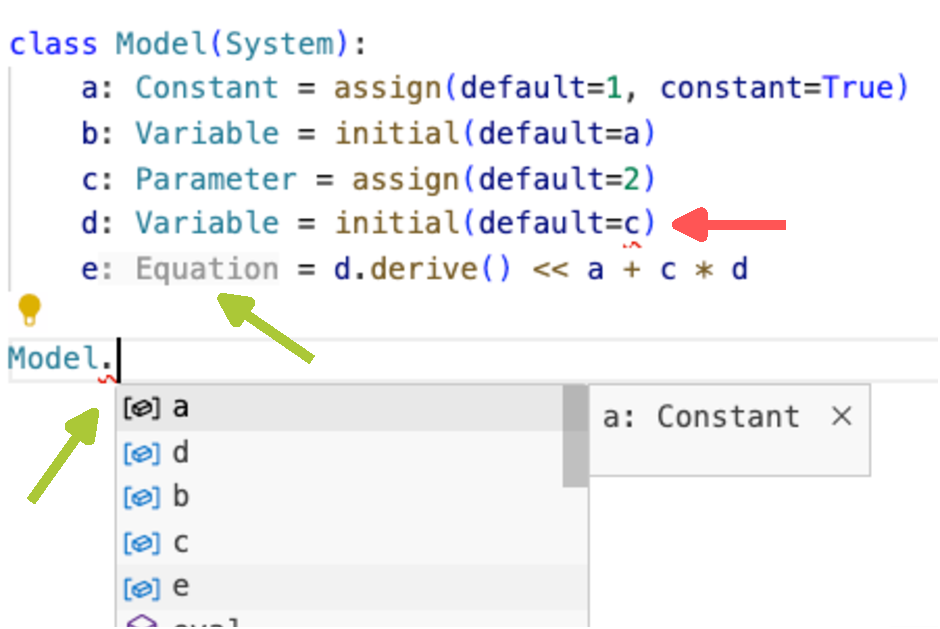
\includegraphics[width=\columnwidth]{ide1.pdf}
  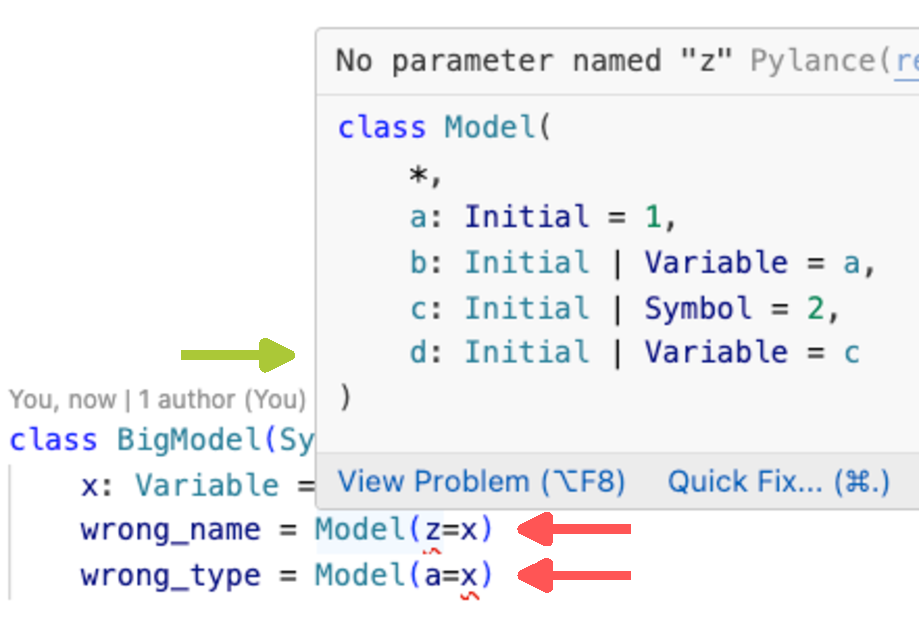
\includegraphics[width=\columnwidth]{ide2.pdf}
  \caption{
    \label{fig-ide}
    Screenshots of Visual Studio Code showing
    tooltips (green arrows) and
    highlighted type errors (red arrows).
    On the left,
    we show that \texttt{a},
    a \texttt{Constant} assigned with \texttt{assign(...,\ constant=True)},
    can be used for \texttt{Variable b}'s initial condition.
    Instead,
    it is flagged as a type error (red underlining)
    when using \texttt{c}, a \texttt{Parameter},
    for \texttt{Variable d}'s initial condition,
    The IDE automatically recognizes \texttt{e} as an \texttt{Equation},
    and provides autocompletion of the \texttt{Model}'s components.
    A tooltip is shown when composing models (green arrow, right),
    which show the expected variables and their default values.
    The IDE highlights wrong names (\texttt{z} is not a name in \texttt{Model})
    and mismatched types (\texttt{x} is \texttt{Variable} and \texttt{a} must be a number or a \texttt{Constant})
  }  
\end{figure}
  
% FIGURE 3
\begin{figure}[t]
  \begin{minipage}[t]{\columnwidth}
    \begin{CodeInput}
    \begin{Highlighting}[]
    \KeywordTok{import} \ClassTok{numpy} \KeywordTok{as} \ClassTok{np}
    \KeywordTok{from} \ClassTok{poincare} \KeywordTok{import} \ClassTok{Simulator}
    
    \VariableTok{sim} \OperatorTok{=} \ClassTok{Simulator}\KeywordTok{(\ClassTok{Oscillator})}
    \VariableTok{df} \OperatorTok{=} \VariableTok{sim}.\FunctionTok{solve}\KeywordTok{(}\VariableTok{save\_at}\OperatorTok{=}\ClassTok{np}.\FunctionTok{linspace}\KeywordTok{(}\ValueTok{0}, \ValueTok{5}, \ValueTok{101}\KeywordTok{))}
    \VariableTok{df}.\FunctionTok{head}\KeywordTok{()}
    \end{Highlighting}
    \end{CodeInput}
    \begin{CodeOutput}
        \begin{tabular}[]{@{}lll@{}}
            \toprule
            & x & v \\
            time & & \\
            \midrule
            0.00 & 1.000000 & 0.000000 \\
            0.05 & 0.998750 & -0.049979 \\
            0.10 & 0.995005 & -0.099835 \\
            0.15 & 0.988772 & -0.149440 \\
            0.20 & 0.980069 & -0.198672 \\
            \botrule
        \end{tabular}
    \end{CodeOutput}
  \end{minipage}%
  \hfill
  \begin{minipage}[t]{\columnwidth}
    \begin{CodeInput}
    \begin{Highlighting}[]
    \VariableTok{df}.\FunctionTok{plot}\KeywordTok{()}
    \end{Highlighting}
    \end{CodeInput}
    %
    \begin{CodeOutput}
      \includegraphics[width=\textwidth]{cell-output}
    \end{CodeOutput}
  \end{minipage}%
  
  \caption{\label{fig-sim}Simulation of the \texttt{Oscillator} system
  from Figure~\ref{fig-second-order}. The output is a
  \texttt{pandas.DataFrame} with a column for each variable and the time
  as index. It is inspected and plotted with the \texttt{pandas} methods.}
\end{figure}
  
  
% FIGURE 4
\begin{figure}[t]
  
    \begin{minipage}[t]{\columnwidth}
      \begin{CodeInput}
      \begin{Highlighting}[]
\KeywordTok{from} \ClassTok{simbio} \KeywordTok{import} (\ClassTok{Compartment}, \ClassTok{MassAction},
                    \ClassTok{Species}, \ClassTok{RateLaw}, \FunctionTok{initial})
      \end{Highlighting}
      \end{CodeInput}
    \end{minipage}%
    \newline
    \begin{minipage}[t]{\columnwidth}
      \begin{minipage}[c]{0.75\columnwidth}
        \begin{CodeInput}
        \begin{Highlighting}[]
\KeywordTok{class}\ClassTok{ Model}\KeywordTok{(}\ClassTok{Compartment}\KeywordTok{)}:
    \CommentTok{"""2A {-}\textgreater{} B"""}

\VariableTok{    A}: \ClassTok{Species }\OperatorTok{=}\FunctionTok{ initial}\KeywordTok{(}\VariableTok{default}\OperatorTok{=}\ValueTok{1}\KeywordTok{)}
\VariableTok{    B}: \ClassTok{Species }\OperatorTok{=}\FunctionTok{ initial}\KeywordTok{(}\VariableTok{default}\OperatorTok{=}\ValueTok{0}\KeywordTok{)}
\VariableTok{    r }\OperatorTok{=}\ClassTok{ RateLaw}\KeywordTok{(}
\VariableTok{        reactants}\OperatorTok{=}\KeywordTok{[}\ValueTok{2} \OperatorTok{*}\VariableTok{ A}\KeywordTok{]},
\VariableTok{        products}\OperatorTok{=}\NormalTok{\KeywordTok{[}B\KeywordTok{]},}
\VariableTok{        rate}\OperatorTok{=}\ValueTok{1}\NormalTok{,}
\KeywordTok{    )}
        \end{Highlighting}
        \end{CodeInput}
      \end{minipage}%
      %
      \begin{minipage}[c]{0.25\columnwidth}
        \centering 
        \[
        \begin{cases}
            \frac{dA}{dt} = -2 \\
            \frac{dB}{dt} = +1
        \end{cases}
        \]
        \[
        \begin{cases}
            A(0) = 1 \\
            B(0) = 0
        \end{cases}
        \]
      \end{minipage}%
    \end{minipage}%
    \newline
    \begin{minipage}[t]{\columnwidth}
        \centering 
        \begin{minipage}[c]{0.75\columnwidth}
\centering 
\begin{CodeInput}
\begin{Highlighting}[]
\KeywordTok{class}\ClassTok{ Model}\KeywordTok{(}\ClassTok{Compartment}\KeywordTok{)}:
    \CommentTok{"""2A {-}\textgreater{} B"""}

\VariableTok{    A}: \ClassTok{Species }\OperatorTok{=}\FunctionTok{ initial}\KeywordTok{(}\VariableTok{default}\OperatorTok{=}\ValueTok{1}\KeywordTok{)}
\VariableTok{    B}: \ClassTok{Species }\OperatorTok{=}\FunctionTok{ initial}\KeywordTok{(}\VariableTok{default}\OperatorTok{=}\ValueTok{0}\KeywordTok{)}
\VariableTok{    r }\OperatorTok{=}\ClassTok{ MassAction}\KeywordTok{(}
\VariableTok{        reactants}\OperatorTok{=}\KeywordTok{[}\ValueTok{2} \OperatorTok{*}\VariableTok{ A}\KeywordTok{]},
\VariableTok{        products}\OperatorTok{=}\NormalTok{\KeywordTok{[}B\KeywordTok{]},}
\VariableTok{        rate}\OperatorTok{=}\ValueTok{1}\NormalTok{,}
\KeywordTok{    )}
            \end{Highlighting}
            \end{CodeInput}
        \end{minipage}%
        %
        \begin{minipage}[c]{0.25\columnwidth}
            \[
            \begin{cases}
                \frac{dA}{dt} = -2 A^2 \\
                \frac{dB}{dt} = +1 A^2
            \end{cases}
            \]
            \[
            \begin{cases}
                A(0) = 1 \\
                B(0) = 0
            \end{cases}
            \]
        \end{minipage}%
    \end{minipage}%
    
    \caption{
      A reaction system for species \(A\) and \(B\)
      with initial conditions \(1\) and \(0\), respectively. A single reaction
      transforming \(2A\) into \(B\) is saved in variable \texttt{r}. The rate
      \(1\) is specified directly for \texttt{RateLaw}, and is proportional to
      the reactants for \texttt{MassAction}.
    }
    \label{fig-simbio}
  \end{figure}
  
  
% FIGURE 5
\begin{figure}[t]
  \centering
  
  \begin{CodeInput}
  \begin{Highlighting}[]
  \KeywordTok{from}\ClassTok{ simbio.io }\KeywordTok{import}\ClassTok{ biomodels, sbml}

  \CommentTok{\# from existing SBML file}
  \VariableTok{model }\OperatorTok{=}\ClassTok{ sbml}.\FunctionTok{load}\KeywordTok{(}\StringTok{"repressilator.sbml"}\KeywordTok{)}
  \CommentTok{\# from BioModels}
  \VariableTok{model }\OperatorTok{=}\ClassTok{ biomodels}.\FunctionTok{load}\KeywordTok{(}\StringTok{"BIOMD12"}\KeywordTok{)}
  \VariableTok{model}
  \end{Highlighting}
  \end{CodeInput}
    
  \begin{CodeOutput}
      \begin{tabular}{@{}lll@{}}
          \multicolumn{3}{l}{Elowitz2000 - Repressilator} \\
          \toprule
          type & total & names \\
          \midrule
          variables  &  6 & PX, PY, PZ, X, Y, Z \\
          parameters & 17 & cell, beta, alpha0, alpha, eff, n, ... \\
          equations  & 12 & Reaction1, Reaction2, Reaction3, ... \\
          \botrule
      \end{tabular}
  \end{CodeOutput}
  
  \caption{Creation of a model from a local SBML file or one uploaded to BioModels.}
  \label{fig-simbio-io}
\end{figure}
    
% FIGURE 6
\begin{figure*}[t]
  \centering
  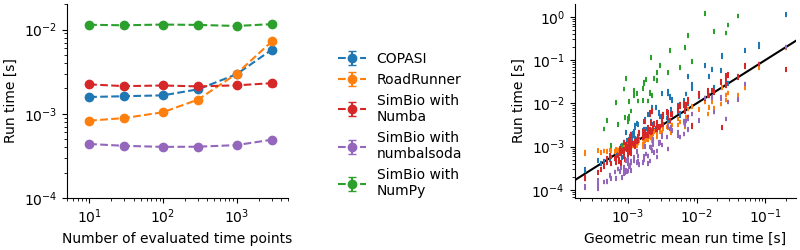
\includegraphics[width=\textwidth]{performance}
  \caption{
    Performance of different softwares to solve models from the curated section of BioModels.
    (left) Run time for the model BIOMD3 as a function of the number of output points.
    (right) Run time for different models for 300 output points,
    using the geometric mean of the different softwares to order them.
    Each point corresponds to the median of 20 runs,
    with a neglibible errorbar given by the interquartile range.
  }
  \label{fig-runtime}
\end{figure*}
  